\documentclass[conference]{IEEEtran}
\IEEEoverridecommandlockouts
% The preceding line is only needed to identify funding in the first footnote. If that is unneeded, please comment it out.
\usepackage{cite}
\usepackage{amsmath,amssymb,amsfonts}
\usepackage{algorithmic}
\usepackage{graphicx}
\usepackage{textcomp}
\usepackage{xcolor}
\usepackage{hyperref}
\def\BibTeX{{\rm B\kern-.05em{\sc i\kern-.025em b}\kern-.08em
    T\kern-.1667em\lower.7ex\hbox{E}\kern-.125emX}}

\hypersetup{      
	urlcolor=blue,
}
\begin{document}

	\title{Conversphere}
	\author{
		\IEEEauthorblockN{1\textsuperscript{st} Feil Lukas}
		\IEEEauthorblockA{
			\textit{OTH Amberg-Weiden} \\
			Bad Kötzting, Deutschland \\
			l.feil@oth-aw.de
		}
		\and
		\IEEEauthorblockN{2\textsuperscript{nd} Markus Fleischmann}
		\IEEEauthorblockA{
			\textit{OTH Amberg-Weiden} \\
			Wernberg-Köblitz, Deutschland\\
			m.fleischmann2@oth-aw.de
		}
		\and
		\IEEEauthorblockN{3\textsuperscript{rd} Stefan Reger}
		\IEEEauthorblockA{
			\textit{OTH Amberg-Weiden} \\
			Schwarzenfeld, Deutschland \\
			s.reger@oth-aw.de
		}
		\and
		\IEEEauthorblockN{4\textsuperscript{th} Lukas Rupp}
		\IEEEauthorblockA{
			\textit{OTH Amberg-Weiden} \\
			Amberg, Deutschland \\
			l.rupp@oth-aw.de
		}
		\and
		\IEEEauthorblockN{5\textsuperscript{th} Sorel Tahata Djoumsi}
		\IEEEauthorblockA{
			\textit{OTH Amberg-Weiden} \\
			Regensburg, Deutschland \\
			s.tahata-djoumsi@oth-aw.de
		}
	}

	\maketitle

	\begin{abstract}
		Web Chat-App mit Raumfunktion und Proximity-Chat
	\end{abstract}

	\begin{IEEEkeywords}
		PWA, Chat, Proximity, Room, Web App, Angular, NodeJS, MongoDB, Express
	\end{IEEEkeywords}

	\section{Einführung}
	Conversphere ist eine Web Chat-Anwendung, die es Benutzern ermöglicht, miteinander zu kommunizieren. Die Kommunikation zwischen den Nutzern erfolgt über Textnachrichten. Es gibt eine Karte, auf welcher die eigene Position auswählbar ist und die Positionen der anderen Nutzern anzeigt. Es können nur die Nachrichten von Benutzern empfangen werden, wenn man innerhalb eines gewissen Umkreises dieser positioniert ist.
	
	Die hörbaren Nachrichten sind in einem Chat-Feld sichtbar. Jede Nachricht ist mit dem Namen des Absenders gekennzeichnet, so dass Nachrichten den verschiedenen Usern zugeordnet werden können. Der Benutzer kann eine Nachricht über ein Textfeld im Chat-Feld senden.
	
	Der Benutzer kann seine Lautstärke der Nachricht wählen (flüstern, normales Gespräch, oder schreien). Dies beeinflusst die Reichweite der Nachricht. Ebenso sind Spezialeffekte wählbar (betrunken, Rage-Mode, usw.), welche die Qualität der Nachricht beeinflussen. Ein Benutzer hat die Möglichkeit, sich ein Profil auf der Seite zu erstellen, um seinen Charakter zu personalisieren. Es können neue Chat-Rooms erstellt werden und man kann schon existierenden Chat-Rooms über deren ID beitreten.
	\ \\

	\section{Motivation}
	Unsere Motivation war es, eine neue Art des Austausches mit unserem einzigartigen Chatroom zu erschaffen. 
	Durch unsere bisherigen Erfahrungen mit den vorhandenen Chats, stießen wir immer wieder auf Langeweile und Unzufriedenheit. Damit waren wir auch nicht allein.
	
	Unser Chatraum soll anders sein als alles, was du bisher erlebt hast.
	
	Durch den individuellen Chat-Radius kann der neuste Klatsch und Tratsch ausgetauscht werden, der vielleicht nicht für jedermann Ohren bestimmt ist. Die Auswahl deiner Chatpartner bietet die perfekte Grundlage dafür. 
	In Zeiten, in welchen Remotearbeit immer essenzieller wird, wollten wir zudem einen sicheren Raum schaffen, in dem es möglich ist, seine Gedanken und Ideen teilen zu können und gleichzeitig sozial distanziert zu bleiben.
	\ \\

	\section{Verwandte Arbeiten}
	Inspiration für das Projekt boten Websites wie Gather \cite{gathertown} oder das mittlerweile beendete Projekt von Skittish \cite{skittish}.
	
	Diese besitzen einen Proximity-Chat bzw. Näherungschat mit Sprachfunktion. Wenn man mit seiner Spielfigur in einer gewissen Entfernung zu anderen Spielern steht kann mit ihnen reden. Verlässt man diesen Umkreis wieder hört man die anderen Spieler nicht mehr.
	
	Dies ist eine gute Möglichkeit für Pandemie-/Quarantänezeiten, um mit Freunde in einer anderen Stadt zu kommunizieren oder um neue Leute kennenzulernen.
	
	Conversphere möchte dieses Grundprinzip als Only-Textchat-Platform adaptieren.
	\ \\

	\section{Alleinstellungmerkmal}
	Conversphere will als möglichst simple und intuitive Chat-Plattform dienen. Da das Design sehr schlicht gehalten wird, hebt sich die Anwendungen vom aktuellen Trend ab, bei welchem immer mehr aufwendige Animationen und Werbung fast schon Standard sind.
	
	Bei Conversphere soll der Austausch im Vordergrund stehen. Da die Anwendung nur Chat-basiert ist, kann sich jeder an Gesprächen beteiligen und muss keine Angst haben, aufgrund von Geschlecht oder Alter anders behandelt zu werden.
	
	Durch das Profil ist es möglich, dass zusätzliche Informationen gespeichert und anderen Nutzern zu Verfügungen gestellt wird. Dadurch ist es für jeden Nutzer selbst frei wählbar, welche Informationen er mit anderen Nutzern teilen möchte. Durch den Verzicht auf Sprach- und Videochats kann man auch völlig anonym mit anderen Nutzern chatten.
	\ \\

	\section{Technisches Grundkonzept}
	\subsection{Datenbank - Mongo DB}
	Zur Speicherung von Nutzer und Spiel bzw. Chatdaten soll eine NoSQL MongoDB Datenbank zum Einsatz kommen. MontoDB Atlas bietet dafür einen kostenlosen Service, welcher eine gehostete MongoDB zu Verfügung stellt.

	\subsection{Backend - Express.js}
	Das Backend soll auf einem in Node.js laufenden Express.js Server basieren. Dieser soll die gesammte Spiellogik implementieren und alle anfallenden Daten zur Speicherung in die Datenbank leiten.

	\subsection{Schnittstellen - Restful API}
	Der Express Server sowie das Frontend sollen über eine Restful API miteinander Kommunizieren. Es sollen dabei für jede Funktion bzw. jede Art von Daten eine eigene Domain sowohl im Frontend als auch im Backend erstellt werden.
	
	\subsection{Frontend - Angular PWA}
	Für das Frontend soll mit Hilfe von Anuglar eine Progressiv Web App erstellt werden welche mit Hilfe einer Render bzw. Animierungsbiliothek erweitert wird.

	\subsection{Deployment - AWS S3 und ECS}
	Die Webseite soll als static Website über AWS S3 an die Clienten verteilt werden. Das Backend soll mit Hilfe eines Docker Containers in der AWS ECS gehostet werden.

	\ \\
	\section{Anforderungen}
	Die Anforderungen werden in Form von User-Storys mit Akzeptanzkriterien formuliert. Die MUSS-Anforderungen definieren das ``Minimum Viable Product`` (MVP). Die SOLL-Anforderungen sollen in den nachfolgenden Iterationen fertiggestellt werden, wobei die Userstorys unter OPTIONAL mögliche Erweiterungen für das Produkt bieten, welche je nach Zeitbedarf umgesetzt werden können.
	\subsection{MUSS-Anforderungen}

	\subsubsection{Raum erstellen}
	\ \\
	Ich als Nutzer möchte über einen Knopf einen neuen Raum erstellen können, um dort einen neuen Chat zu starten, welcher am Anfang bis auf mich leer ist.
	
	\textbf{Akzeptanzkriterien:}
	\begin{itemize}
		\item Eingabe des Nicknames, mit welchen man im Raum angezeigt wird.
		\item Weiterleitung in neuen Raum nach Button-Druck
		\item Anzeige der Raum-ID für diesen Raum
		\item Chatroom wird angezeigt
	\end{itemize}
	\ \\
	\subsubsection{Raum beitreten}
	\ \\
	Ich als Nutzer möchte nach Erhalt eines Codes durch einen anderen Spieler nach Eingabe des Codes mittels einem Knopfdruck dessen Raum beitreten, um dort an dem Chat teilzunehmen.
	
	\textbf{Akzeptanzkriterien:}
	\begin{itemize}
		\item Eingabe des Nicknames, mit welchen man im Raum angezeigt wird.
		\item Nach Eingabe der Raum-ID  wird bei einem ungültigen Wert eine Meldung an den Nutzer ausgegeben.
		\item Bei einer gültigen Raum-ID wird man in den Raum weitergeleitet.
		\item Chatroom wird angezeigt
	\end{itemize}
	\ \\
	\subsubsection{Schreiben von Nachrichten}
	\ \\
	Ich als Nutzer möchte über eine Chatbox Nachrichten eingeben können.
	
	\textbf{Akzeptanzkriterien:}
	\begin{itemize}
		\item Die Nachricht wird im Textfeld angezeigt.
		\item Das Textfeld soll die letzten 10 Nachrichten anzeigen. Mit einem Schieberegler kann die Anzahl der Nachrichten, welche angezeigt werden, verändert werden.
	\end{itemize}
	
	\ \\
	\subsubsection{Bewegen auf der Karte}
	\ \\
	Ich als Nutzer möchte mich auf der Karte bewegen können.
	
	\textbf{Akzeptanzkriterien:}
	\begin{itemize}
		\item Der Spieler kann seine Position mit einem Klick auf der Karte auswählen.
		\item Die Position soll auf der Karte sichtbar sein.
		\item Der Spieler kann seine Position jederzeit ändern.
		\item Der Spieler soll jederzeit seine Position auf der Karten sowie die Position andere Spieler sehen können.
	\end{itemize}
	
	\ \\
	\subsection{SOLL-Anforderungen}
	\subsubsection{Lautstärke der Nachricht einstellen}
	\ \\
	Ich als Nutzer möchte über einen Schieberegler einstellen können, wie weit man meine Nachrichten lesen kann.
	
	\textbf{Akzeptanzkriterien:}
	\begin{itemize}
		\item Reichweite einstellbar über den Schieberegler.
		\item Nach verschieben ändert sich der Umkreis.
	\end{itemize}
	\ \\
	
	\subsubsection{Darstellung der Nachricht}
	\ \\
	Ich als Nutzer möchte, dass je nach Lautstärke der erreichten Nachrichten diese in unterschiedlicher Weise angezeigt werden, so dass es leichter erkennbar ist, welche Nachrichten von Spieler im näheren Umkreis stammen.
	
	\textbf{Akzeptanzkriterien:}
	\begin{itemize}
		\item Je nach Entfernung und Lautstärke der Nachricht wird diese mit unterschiedlichem Verblassungs-Effekt angezeigt.
	\end{itemize}
	\ \\

	\subsubsection{Drunk-Mode}
	\ \\
	Ich als Nutzer möchte einen Drunk-Mode, in welchem Nachrichten in welchem Buchstaben zufällig vertauscht werden.
	
	\textbf{Akzeptanzkriterien:}
	\begin{itemize}
		\item Aktivierung des Drunk-Modes über einen Button im Chat-Feld.
		\item Nachrichten im Drunk-Mode werden den mit zufällig vertauschten Buchstaben innerhalb eines Wortes angezeigt.
	\end{itemize}
	
	\subsubsection{Rage-Mode}
	\ \\
	Ich als Nutzer möchte einen Rage-Mode, in ich meine Nachricht an alle Teilnehmer im Raum senden kann.
	
	\textbf{Akzeptanzkriterien:}
	\begin{itemize}
		\item Durch das senden einer Nachricht im CAPS-Lock wird der Rage-Mode aktiviert.
		\item Die gesendete Nachricht ist für alle Nutzer sichtbar.
	\end{itemize}
	

\ \\

	\subsection{OPTIONAL-Anforderungen}
	\subsubsection{Registrieren}
	\ \\
	Ich als nicht registrierter Nutzer möchte eine Möglichkeit besitzen, mich zu registrieren, um mein Profil dauerhaft speicher zu können.
	
	\textbf{Akzeptanzkriterien:}
	\begin{itemize}
		\item Button ``Registrieren`` leitet an das Formular mit den Angaben weiter
		\item Formular frägt folgen Werte ab: E-Mail und Nutzername (müssen eindeutig sein) und Passwort
		\item Nach Prüfung, ob die E-Mail und der Nutzernamen eindeutig sind, wird eine Bestätigungsmail versendet
		\item Erst nach Bestätigung wird der Account freigeschaltet
	\end{itemize}
	
	\ \\
	\subsubsection{Anmelden}
	\ \\
	Ich als registrierter Nutzer möchte eine Möglichkeit besitzen, mich anzumelden, um auf meinen Account zuzugreifen.
	
	\textbf{Akzeptanzkriterien:}
	\begin{itemize}
		\item Button ``Login`` leitet an ein Formular für die Eingabemöglichkeit der E-Mail/Nutzernamen und des Passworts weiter
		\item Nach erfolgreicher Eingabe wieder Weiterleitung auf den Startbildschirm, jedoch ist erkennbar, dass man eingeloggt ist
	\end{itemize}
	
	\ \\
	\subsubsection{Nutzerprofil bearbeiten}
	\ \\
	Ich als angemeldeter Nutzer möchte eine Möglichkeit besitzen, dass ich auf meine Profilseite zugreifen kann, und dort Eigenschaften wie Nickname, Uhrzeit/Ort einstellen kann.
	
	\textbf{Akzeptanzkriterien:}
	\begin{itemize}
		\item Button ``Profil`` leitet auf die Profilseite weiter
		\item Eigenschaften werden angezeigt
		\item Bei Änderungen an den Eigenschaften wird der ``Speichern``-Button aktiv
		\item Nur bei der Betätigung des ``Speichern``-Buttons werden die Änderungen gespeichert, ansonsten verworfen
		\item Wird die Profilseite verlassen, ohne dass Änderungen gespeichert sind, so wird der Nutzer darauf aufmerksam gemacht
	\end{itemize}
	
	\begin{figure}[htbp]
		\centering
		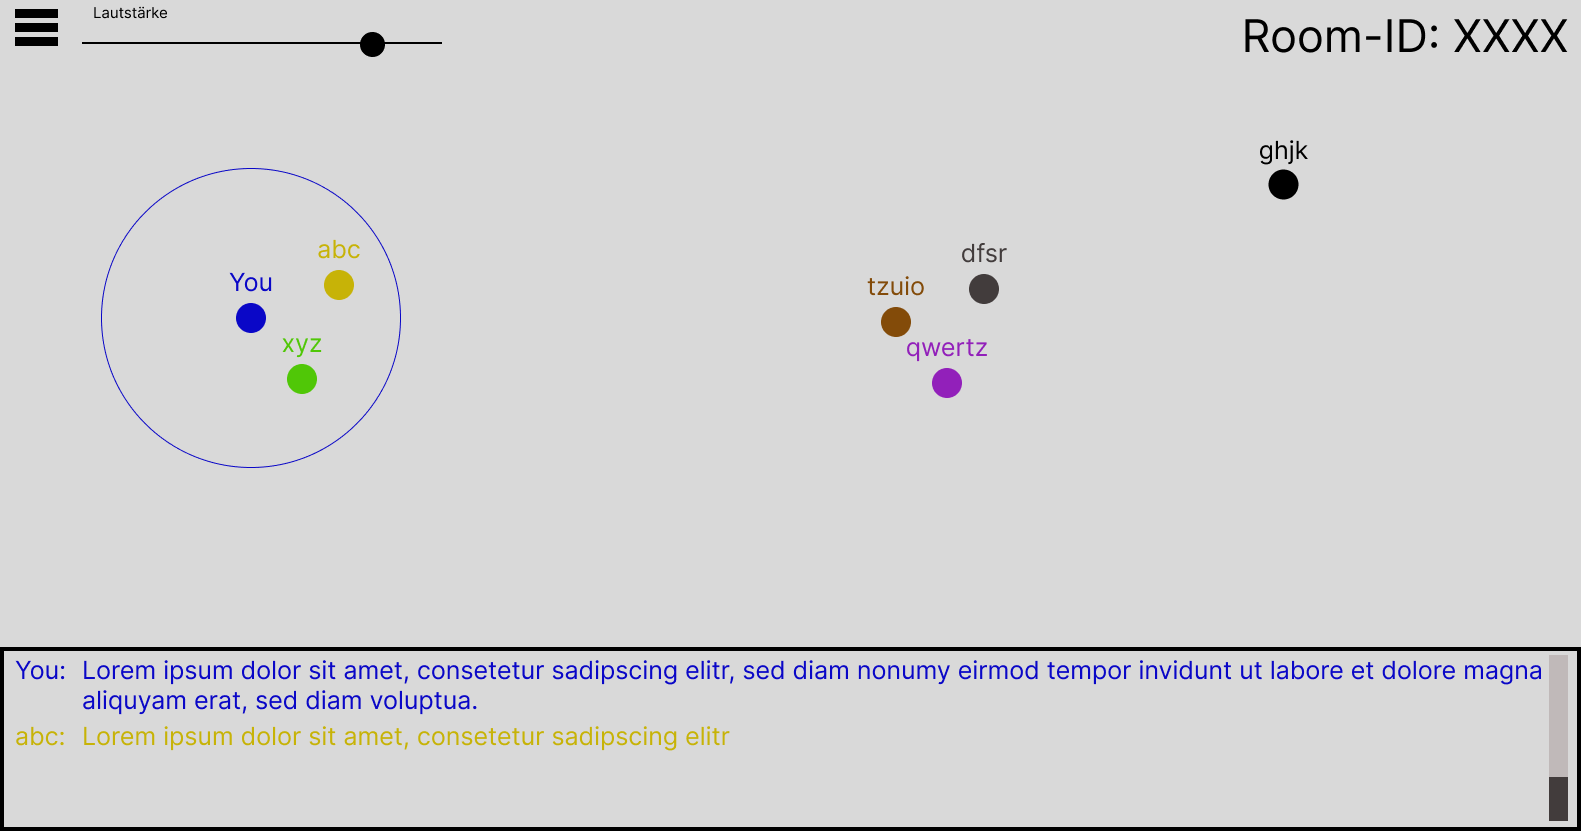
\includegraphics[width=\linewidth]{skizze.png}
		\caption{Skizze eines Chat-Rooms}
	\end{figure}
	
	
	\begin{thebibliography}{99}
		
	\bibitem{gathertown} \url{https://www.gather.town/} 
	\bibitem{skittish} \url{https://skittish.com/}
	
	
	\end{thebibliography}

\end{document}